\subsection{Rod Cusping Description}
\begin{frame}

\begin{columns}
\begin{column}{0.6\textwidth}
    \begin{itemize}
        \item Nodes must be axially homogeneous
        \item Control rod positions often do not align with node boundaries, 
        requiring homogenization of control rod and moderator
        \item Volume homogenization preserves material volume/mass, but not 
        reaction rates
        \item Two approaches to prevent rod cusping:
        \begin{itemize}
          \item Refine mesh to align with all control rod positions
          \item Decusping method to improve homogenization
        \end{itemize}
    \end{itemize}
\end{column}
\begin{column}{0.4\textwidth}
\begin{figure}[h]
  \centering
  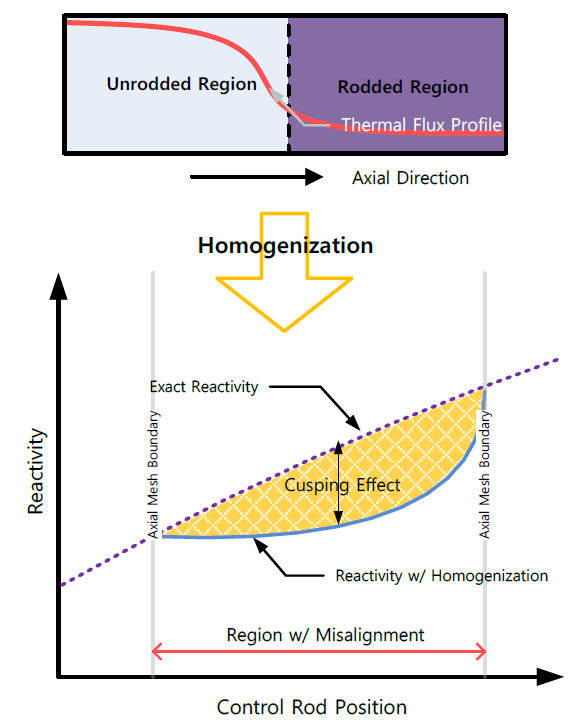
\includegraphics[width=\textwidth]{cusping_effect_Joo.png}
\end{figure} 
\end{column}
\end{columns}
    
\end{frame}

%%%%%%%%%%%%%%%%%%%%%%%%%%%%%%%%%%%%%%%%%%%%%%%%%%%%%%%%%%%%%%%%%%%%%%%%%%%%%%%%%

\begin{frame}
    
\begin{center}
    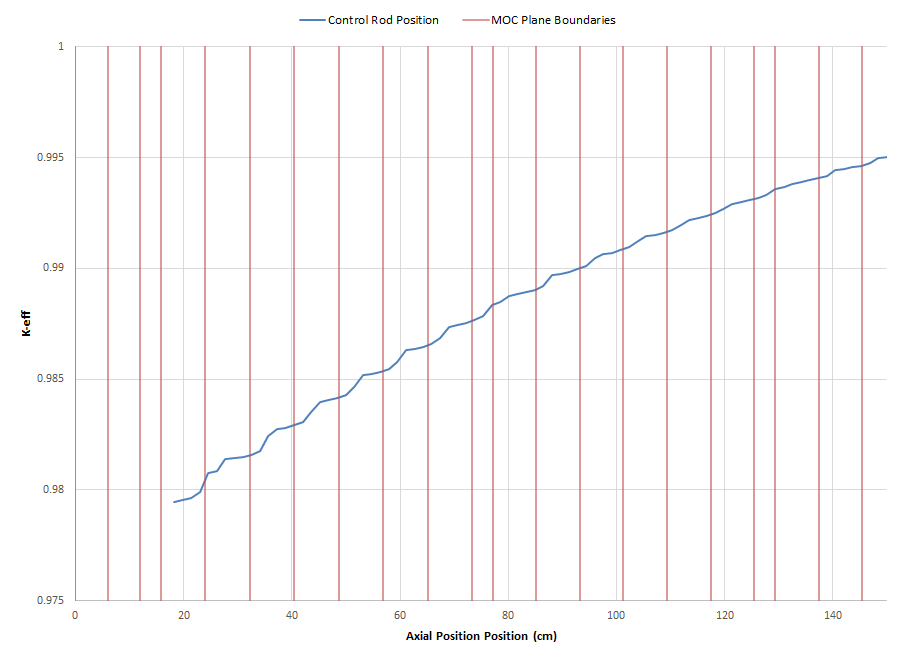
\includegraphics[width=0.8\textwidth]{p4cuspingEffects.png}
\end{center}
\vfill
    
\end{frame}

%%%%%%%%%%%%%%%%%%%%%%%%%%%%%%%%%%%%%%%%%%%%%%%%%%%%%%%%%%%%%%%%%%%%%%%%%%%%%%%%%

\begin{frame}[t]{Methods Shortcomings}
    
    \begin{itemize}
        \item Extensive research has been done on decusping methods, primarily for nodal codes
        \item Several methods have been developed for 2D/1D codes
        \begin{itemize}
            \item Some methods involved coarse approximations with limited accuracy
            \item Others required expensive additional calculations that increased runtime of the code significantly
        \end{itemize}
        \item New methods need to improve on prior ones by providing more accurate solutions without significantly slowing down calculations
    \end{itemize}

\end{frame}